\documentclass[../defence.tex]{subfiles}

\begin{document}
  \begin{frame}{ALD for smaller pore diameters II}
    \begin{columns}[onlytextwidth, T]
      \column{\dimexpr\linewidth / 21 * 12}
        \scalebox{0.55}{
          \tikzsetnextfilename{295d_250ALD}
          \begin{tikzpicture}
              \def\PrelMin{.5}
      				\def\PrelMax{1}
      				\def\TransMin{1e-2}
      				\def\TransMax{1}
      				\def\LfMin{0}
      				\def\LfMax{2}
              %
              \begin{axis}[
                /tikz/line join=bevel,
                grid,
      					axis y line*=left,
                legend style={at={(0,0.5)}, legend columns=1, anchor=north west},
                every axis plot,
      					axis y line*=left,
      					line width = 1pt,
      					xmin = \PrelMin, xmax = \PrelMax,
      					ymin = \LfMin, ymax = \LfMax,
      					xlabel = {Relative pressure $P_\mathrm{rel}$},
      					ylabel = {Liquid fraction $LF$},
      					ytick = {0,0.25,0.50,0.75,1},
                ]
      					% Add plots
      					\addplot[mark=none, color=red] table [x=Prel,y=liquid_fraction]{tikz/graphs/295d_ALD/295d250ALD_cond_1.txt};
      					%\addlegendentry{$LF_\mathrm{cond}^\mathrm{295d''}$}
      					\addplot[mark=none, color=blue!50] table [x=Prel,y=liquid_fraction]{tikz/graphs/295d_ALD/295d250ALD_evap_1.txt};
      					%\addlegendentry{$LF_\mathrm{evap}^\mathrm{295d''}$}
              \end{axis}
      				% transmission
      				\begin{axis}[
                /tikz/line join=bevel,
      					ymode=log,
      					axis y line*=right, ylabel near ticks, yticklabel pos=right,
      					line width = 1pt,
      					xmin = \PrelMin, xmax = \PrelMax,
      					ymin = \TransMin, ymax = \TransMax,
      					ylabel = {Transmission $T$},
      					xtick = {1e-1,1e-2,1e-3},
      					ytick = {1,1e-1},
                ymajorgrids=true,
                legend style={at={(0,0.5)}, legend columns=1, anchor=west},
      					]
      					% Add plots
      					\addplot[mark=none, color=red] table [x=Prel,y=transmission]{tikz/graphs/295d_ALD/295d250ALD_cond_1.txt};
      					\addlegendentry{Condensation}
      					\addplot[mark=none, color=blue!50] table [x=Prel,y=transmission]{tikz/graphs/295d_ALD/295d250ALD_evap_1.txt};
      					\addlegendentry{Evaporation}
      				\end{axis}
          \end{tikzpicture}}
        \pause

      \column{\dimexpr\linewidth / 21}
      \column{\dimexpr\linewidth / 21 * 8}
        \vfill
        \scalebox{0.5}{
          \tikzsetnextfilename{ald_rate}
          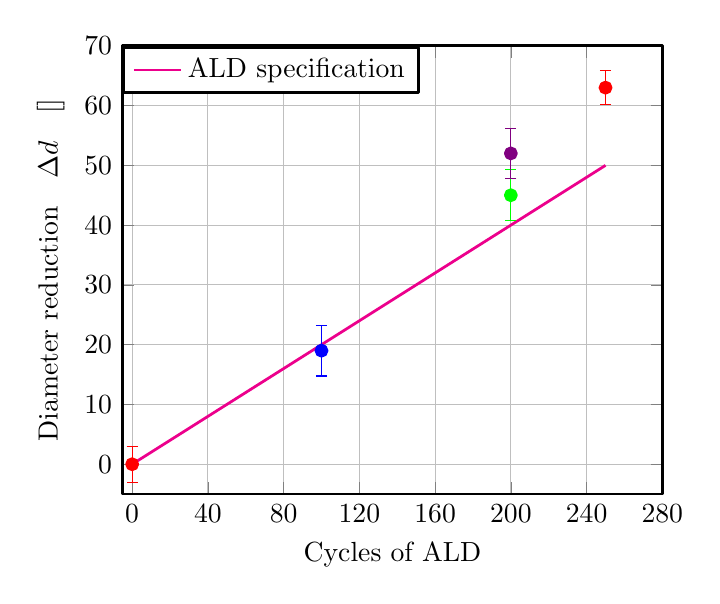
\begin{tikzpicture}
                \def\Xmin{-5}
                \def\Xmax{280}
                \def\Ymin{-5}
                \def\Ymax{70}
                \begin{axis}
                    [
                    /tikz/line join=bevel,
                    line width = 1pt,
                    xmin = \Xmin, xmax = \Xmax,
                    ymin = \Ymin, ymax = \Ymax,
                    xlabel = {Cycles of ALD},
                    ylabel = {Diameter reduction$\quad \Delta d\quad[\si{\nano\meter}]$},
                    xtick = {0,40,80,120,160,200,240,280},
                    ytick = {0,10,20,30,40,50,60,70},
                    grid,
                    legend style={at={(0,1)}, legend columns=1, anchor=north west},
                    ]
                    %\addplot [color=blue, only marks,mark=o,]
                    % plot [error bars/.cd, y dir = both, y explicit]
                    % table[x=cycles, y=reduction, y error=error]{ALD_data.txt};
                    \addplot[color=magenta, mark=none]
                    coordinates {
                    (0,0)
                    (250,50)};
                    \addlegendentry{ALD specification}
                    \addplot [color=red, only marks, mark=*, mark options={solid},  error bars/.cd, y dir = both, y explicit]
                    coordinates {
                    (0, 0) +- (0,3)};
                    \addplot [color=blue, only marks, mark=*, mark options={solid}, error bars/.cd, y dir = both, y explicit]
                    coordinates {
                    (100, 19) +- (0,4.24)};
                    \addplot [color=green, only marks, mark=*, mark options={solid},  error bars/.cd, y dir = both, y explicit]
                    coordinates {
                    (200, 26+19) +- (0,4.24)};
                    \addplot [color=violet, only marks, mark=*, mark options={solid}, error bars/.cd, y dir = both, y explicit]
                    coordinates {
                    (200, 52) +- (0,4.24)};
                    \addplot [color=red, only marks, mark=*, mark options={solid},  error bars/.cd, y dir = both, y explicit]
                    coordinates {
                    (250, 63) +- (0,2.83)};
                \end{axis}
          \end{tikzpicture}}
    \end{columns}
  \end{frame}
\end{document}
